\hypertarget{orconveyormovement.cpp-example}{
\subsection{orconveyormovement.cpp}
}
\begin{DoxyAuthor}{Author}
Rosen Diankov
\end{DoxyAuthor}
 
\begin{DoxyImage}
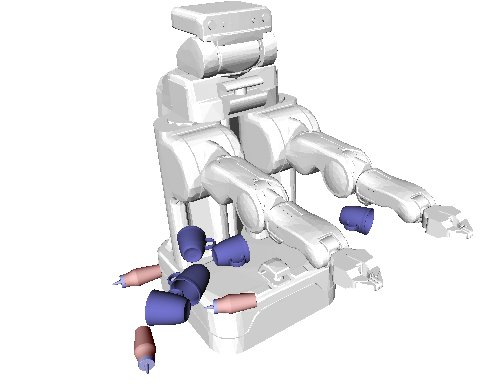
\includegraphics[width=10cm]{cppexample_orconveyormovement.jpg}
\caption{Parts moving on a conveyor belt.}
\end{DoxyImage}


Shows how to setup a simulation loop to move objects around a conveyor belt.

{\bfseries Full Example Code:}


\begin{DoxyCodeInclude}

#include <openrave-core.h>
#include <vector>
#include <sstream>
#include <boost/thread/thread.hpp>
#include <boost/bind.hpp>

using namespace OpenRAVE;
using namespace std;

#ifdef _WIN32
#define WIN32_LEAN_AND_MEAN
#include <windows.h>
#define usleep(micro) Sleep(micro/1000)
#endif

class ConveyorBeltModule : public ModuleBase
{
    struct RegisteredBody
    {
        string filename;
        dReal appearanceprobability;     // probably of appearance in 1 second
    };

    struct InstancedBody
    {
        KinBodyPtr pbody;
        dReal timeleft;
    };
    SpaceSamplerBasePtr _psampler;
public:
    ConveyorBeltModule(EnvironmentBasePtr penv, std::istream& is) : ModuleBase(pe
      nv)
    {
        __description = "Handles conveyor belt movement";
        RegisterCommand("registerbody",boost::bind(&ConveyorBeltModule::RegisterB
      ody,this,_1,_2),"registers a body to be put into the environment");
        movevel = Vector(0,0.4,0);
        start = Vector(0.5,-1,0.6);
        _psampler = RaveCreateSpaceSampler(penv,"mt19937");
    }

    int main(const string& cmd)
    {
        return 0;
    }

    bool RegisterBody(ostream& sout, istream& sinput)
    {
        EnvironmentMutex::scoped_lock lock(GetEnv()->GetMutex());
        RegisteredBody body;
        sinput >> body.filename >> body.appearanceprobability;
        if( !sinput ) {
            return false;
        }
        _listregistered.push_back(body);
        return true;
    }

    bool SimulationStep(dReal fElapsedTime)
    {
        for(list<RegisteredBody>::iterator it = _listregistered.begin(); it != _l
      istregistered.end(); ++it) {
            // appearanceprobabiliy is in seconds, so have to transform
            dReal appearanceprobability = 1-pow(1-it->appearanceprobability,fElap
      sedTime);
            vector<dReal> vsample;
            _psampler->SampleSequence(vsample,4,IT_OpenStart);
            if( vsample.at(0) < appearanceprobability ) {
                KinBodyPtr pbody = GetEnv()->ReadKinBodyXMLFile(it->filename);
                GetEnv()->AddKinBody(pbody,true);
                InstancedBody b;
                for(int iter = 0; iter < 10; ++iter) {
                    Transform t;
                    t.rot = geometry::quatFromAxisAngle<dReal>(Vector(0,0,1),vsam
      ple.at(1)*2*PI);
                    t.trans = start + Vector(vsample.at(2)-0.5,vsample.at(3)-0.5,
      0)*0.4;
                    pbody->SetTransform(t);
                    if( !GetEnv()->CheckCollision(KinBodyConstPtr(pbody)) ) {
                        b.pbody = pbody;
                        break;
                    }
                }

                if( !b.pbody ) {
                    GetEnv()->Remove(pbody);
                }
                else {
                    b.timeleft = 4.0;
                    _listinstances.push_back(b);
                }
            }
        }

        list<InstancedBody>::iterator it = _listinstances.begin();
        while(it != _listinstances.end() ) {
            Transform t = it->pbody->GetTransform();
            t.trans += fElapsedTime*movevel;
            it->pbody->SetTransform(t);
            it->timeleft -= fElapsedTime;
            if( it->timeleft <= 0 ) {
                GetEnv()->Remove(it->pbody);
                it = _listinstances.erase(it);
            }
            else {
                ++it;
            }
        }
        return false;
    }

    static InterfaceBasePtr create(EnvironmentBasePtr penv, std::istream& is)
    {
        return InterfaceBasePtr(new ConveyorBeltModule(penv,is));
    }

private:
    Vector start, movevel;
    list<RegisteredBody> _listregistered;
    list<InstancedBody> _listinstances;
};

void SetViewer(EnvironmentBasePtr penv, const string& viewername)
{
    ViewerBasePtr viewer = RaveCreateViewer(penv,viewername);
    penv->AddViewer(viewer);
    viewer->main(true);
}

int main(int argc, char ** argv)
{
    // initialize openrave and register the conveyor module
    RaveInitialize(true);
    boost::shared_ptr<void> handle = RaveRegisterInterface(PT_Module,"conveyorbel
      t",OPENRAVE_MODULE_HASH,OPENRAVE_ENVIRONMENT_HASH,ConveyorBeltModule::create);
    EnvironmentBasePtr penv = RaveCreateEnvironment();

    // load the environment
    string scenefilename = "robots/pr2-beta-static.zae";
    string viewername = "qtcoin";
    boost::thread thviewer(boost::bind(SetViewer,penv,viewername)); // create the
       viewer
    penv->Load(scenefilename);

    // create the conveyor module and add a couple of bodies for simulation
    ModuleBasePtr p = RaveCreateModule(penv,"conveyorbelt");
    penv->AddModule(p,"");
    stringstream sout, sin("registerbody data/mug1.kinbody.xml 0.6");
    p->SendCommand(sout,sin);
    sin.clear();
    sin.str("registerbody data/ketchup.kinbody.xml 0.3");
    p->SendCommand(sout,sin);

    thviewer.join(); // wait for the viewer thread to exit
    penv->Destroy(); // destroy
    return 0;
}
\end{DoxyCodeInclude}
 